\documentclass{beamer}

%%% Dichiarazione dei pacchetti standard.
\usepackage[italian]{babel}
\usepackage[utf8x]{inputenc}
\usepackage{graphicx}
\usepackage{xymtex}
\usepackage{natbib}

%%% Personalizzazione del layout---articolata su cinque livelli.
\usetheme{Warsaw}        % layout complessivo. 
\useinnertheme{default} % layout interno.
\useoutertheme{default} % layout esterno.
\usecolortheme{default} % schema di colori.
\usefonttheme{default}  % schema dei font.
% Inutile dire che se volete tutti i default, potete risparmiarvi gli ultimi
% quattro comandi. 

%%% Titolo e autore.
\title{I motivi delle proteine}
\subtitle{Dalla struttura {\tt secodaria} alla {\tt supersecondaria}}
\author{Ilario Gelmetti}
\institute{Università di Pisa}
\date{\today}

\def\newblock{\hskip .11em plus .33em minus .07em} 
\beamersetuncovermixins{\opaqueness<1>{25}}{\opaqueness<2->{15}}
\graphicspath{ {./img/} }

\begin{document}

\begin{frame}
  \titlepage
\end{frame}


\section[Sommario]{}
\begin{frame}
\tiny{\tableofcontents}
\end{frame}


\section{Introduzione}
\begin{frame}
  \frametitle{Introduzione}
  \framesubtitle{L'importanza dei motivi}
 
  \begin{itemize}
   \item 	La struttura secondaria di una proteina è la conformazione tridimensionale \emph{locale} di un suo segmento.
  \begin{itemize}
    \item Formalmente è definita dai legami ad idrogeno tra i gruppi ammidici e carbonilici della catena principale.
    \end{itemize}
\end{itemize}\uncover<3->{
\begin{figure}

\centering
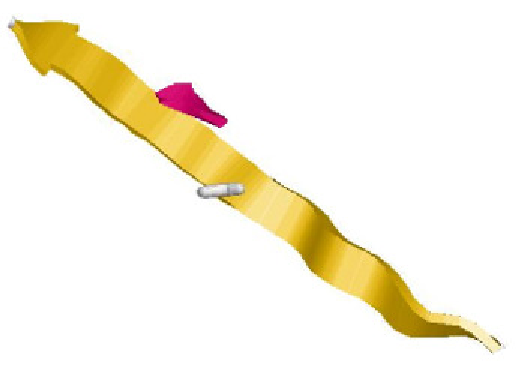
\includegraphics[scale=0.5]{betastrand.pdf}\caption{Un filamento $\beta$ costituito da 11 amminoacidi\citep{PDB}}\label{bstrand}
\end{figure}}


\end{frame}
\begin{frame}
  \begin{itemize}
  \item  	Un \emph{motivo} è una struttura \emph{supersecondaria} ossia una combinazione di elementi di struttura secondaria.
\end{itemize}\uncover<3->{
\begin{figure}

\centering
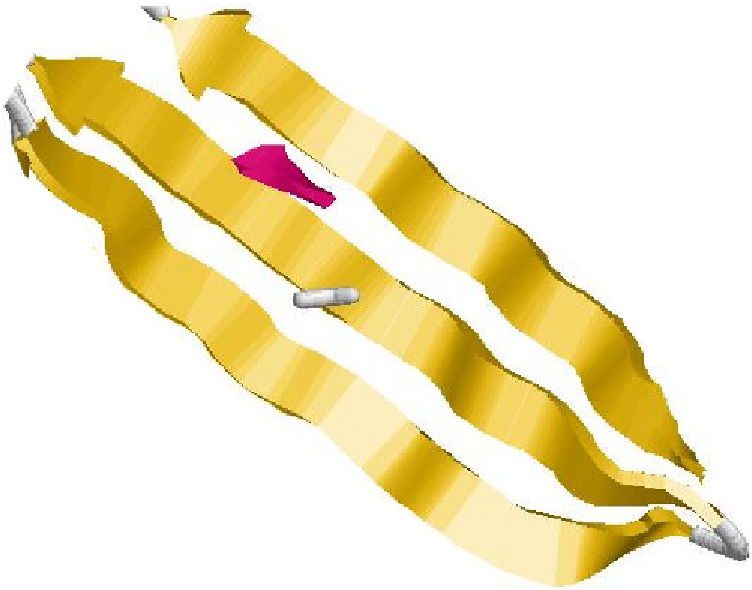
\includegraphics[scale=0.5]{psiloop.pdf}\caption{Un motivo $\psi loop$ costituito da 3 filamenti $\beta$\citep{PDB}}\label{psiloop}
\end{figure}}

\end{frame}
\begin{frame}
  \begin{itemize}
  \item   	Le proteine hanno funzioni diverse in base ai domini\footnote{Un dominio è una parte di proteina che può ripiegarsi in modo stabile anche se isolata in soluzione.} 
		in esse contenuti e, spesso ma non sempre, i domini contengono motivi noti e ricorrenti.
\end{itemize}\uncover<3->{
   \begin{figure}

\centering
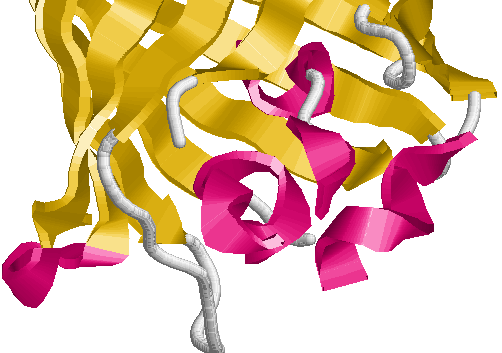
\includegraphics[scale=0.25]{terziaria.png}\caption{Un $\beta$ barile e delle $\alpha$ eliche facenti parte della \emph{Green fluorescent protein}\citep{PDB}}\label{bbarrel}
\end{figure} }

\end{frame}


\section{Interazioni}
\subsection{Legami ad idrogeno}
\begin{frame}
  \frametitle{Struttura secondaria}
  \framesubtitle{Legami ad idrogeno}
Per identificare i legami ad idrogeno è utilizzata la definizione DSSP\footnote{Dictionary of Protein Secondary Structure} che utilizza il valore di:
$$ E = q_{1} q_{2} \left\{ \frac{1}{r_{ON}} +  \frac{1}{r_{CH}} - \frac{1}{r_{OH}} - \frac{1}{r_{CN}} \right\}  $$
in cui si considera il carattere elettrostatico mentre un legame ad idrogeno ha anche caratteristiche da legame covalente: \pause
  \begin{enumerate}
  \item Direzionalità\pause
  \item Forza: da 5 a 30 $kJ/mole$ maggiore di una interazione di van der Waals, minore di un legame covalente o ionico\pause
  \item Distanze: minori della somma dei raggi di van der Waals\pause
  \item Coinvolge un numero limitato di atomi: si possono osservare legami ad idrogeno a più centri
  \end{enumerate}

\end{frame}

\subsection{Interazioni idrofobiche}
\begin{frame}
  \frametitle{Struttura terziaria}
  \framesubtitle{Interazioni idrofobiche}
  Le interazioni idrofobiche sono importanti per la struttura terziaria e quaternaria. Permettono di avere un \emph{core idrofobico} 
in cui si troveranno principalmente gli amminoacidi apolari come:\pause
\changeunitlength{0.06pt}
\tetramethylenei {1==CH$_3$;4==OH} {2SB==NH$_2$;2SA==H;3D==O}
\pentamethylene{5==OH}{2==\null;3SB==NH$_2$;3SA==H;4D==O}
\hexamethylenei{6==OH}{2==\null;4SB==NH$_2$;4SA==H;5D==O}
\hexamethylenei{6==OH}{3A==\null;4SB==NH$_2$;4SA==H;5D==O}
\tetramethylenei{4==OH}{1W==\bzdrv[A]{2==(yl)};2SB==NH$_2$;2SA==H;3D==O}
\heptamethylene{1==CH$_3$;2==S;7==OH}{5SB==NH$_2$;5SA==H;6D==O}\\ \pause
La \emph{driving force} di questa interazione è il guadagno entropico che si ha nell'espellere le molecole di acqua; 
la variazione di entalpia invece è leggermente favorevole alla solvatazione.

  
\end{frame}

\subsection{Ponti salini}
\begin{frame}
  \frametitle{Struttura terziaria}
  \framesubtitle{Ponti salini}
  
\begin{itemize}
  \item   Solitamente le interazioni ioniche sono accompagnate da un legame ad idrogeno.
  \end{itemize}\pause
\begin{figure}
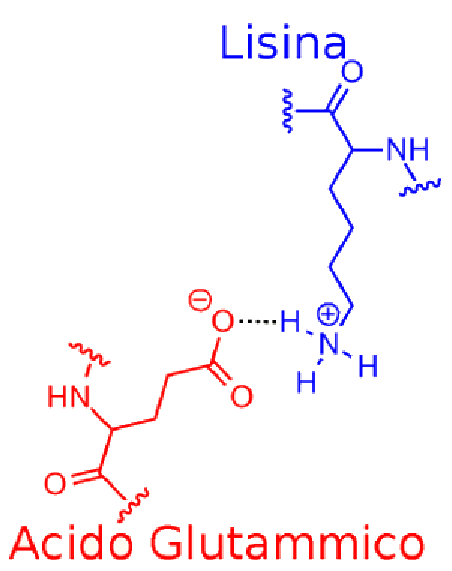
\includegraphics[scale=0.4]{salt_bridge.pdf}\caption{Un ponte ionico con legame ad H}\label{saltbridge}
\end{figure}

\end{frame}
\begin{frame}
\begin{itemize}
  \item	La distanza tra i residui partecipanti deve essere inferiore a 4.0 \AA.\citep{electrointeract} \pause
  \item I residui che danno queste interazioni sono: \emph{acido aspartico, acido glutammico , lisina, arginina.} \\
\changeunitlength{0.06pt}

\hexamethylenei{1==HO;6==OH}{2D==O;4SB==NH$_2$;4SA==H;5D==O}
\heptamethylene {1==HO;7==OH} {2D==O;5SB==NH$_2$;5SA==H;6D==O}
\octamethylenei{1==NH$_2$;8==OH}{6SB==NH$_2$;6SA==H;7D==O}
\pause
  \item In dipendenza dal $pH$ e dai fattori che influenziano il $pK_a$: \emph{istidina, tirosina, serina. }  \\
\begin{figure}
 


\begin{picture}(1300,500)\tetramethylenei{4==OH}{1W==\fiveheterovi[A]{1==N;4==N}{1==H;2==(yl)};2SB==NH$_2$;2SA==H;3D==O}\end{picture}
 \begin{picture}(900,500)\tetramethylenei{4==OH}{1W==\bzdrv[c]{5==OH;2==(yl)};2SB==NH$_2$;2SA==H;3D==O}\end{picture}                                                                                                      
\begin{picture}(900,600) \pentamethylene{1==HO;5==OH}{3SB==NH$_2$;3SA==H;4D==O}\end{picture}

\end{figure}
  \end{itemize}

\end{frame}

\subsection{Legami disolfuro}
\begin{frame}
  \frametitle{Struttura terziaria}
  \framesubtitle{Legami disolfuro}
  
  \begin{enumerate}
  \item  È un legame covalente con un energia di legame di $60 kcal/mol$.\pause
  \item  Si forma come deidrogenazione di due residui di cisteina. 
\changeunitlength{0.07pt}
\pentamethylene{1==HS;5==OH}{3SB==NH$_2$;3SA==H;4D==O}\pause
  \item  Il citosol è un ambiente riducente perciò il legame disolfuro è instabile. \pause
  \item  L'angolo diedro tende ad essere di $\pm90°$.
\end{enumerate}
\end{frame}

\begin{frame}
  \begin{enumerate}
  \item  Il legame disolfuro può fungere da nucleo idrofobico.\pause
  \item  Per il punto sopra e a causa dell'avvicinamento delle due catene si viene a espellere l'acqua favorendo così la formazione dei legami ad idrogeno che costituiscono la struttura secondaria.\pause 
  \item  Una volta formati dei legami disolfuro, a $pH$ alti si può avere uno scambio di legami disolfuro per attacco di un tiolato.
\end{enumerate}
 

\end{frame}

\subsection{Modifiche post-traduzionali}
\begin{frame}  
  \frametitle{Struttura terziaria}
  \framesubtitle{Modifiche post-traduzionali}
  I legami disolfuro sono un esempio di \emph{modifica post-traduzionale}.
Le P.T.M. più comuni sono:
\begin{itemize}
 \item Modifiche strutturali.
\begin{itemize}
 \item Legami disolfuro.
\item Rottura del legame peptidico.
\item Racemizzazione della \emph{prolina}.
\end{itemize}
 

\item Addizione di gruppi funzionali.
\item Addizione di altri peptidi.
\item Modifica dell'amminoacido presente.
\end{itemize}
\end{frame}


\section{Strutture secondarie}
\subsection{Strutture secondarie elicoidali}
\begin{frame}
\frametitle{Strutture secondarie}
  \framesubtitle{Strutture secondarie elicoidali}
  Il legame ad idrogeno intracatena si può formare tra un carbonile e i gruppi amminici successivi nella catena, 
ad ognuno di questi corrisponde una struttura secondaria:

\begin{itemize}
\uncover<2->{ \item $1\rightarrow7$ Nastro $2_7$ - filamento $\beta$}
\uncover<3->{ \item $1\rightarrow10$ Elica $3_{10}$}
\uncover<4->{ \item $1\rightarrow13$ Elica $3.6_{13}$ - $\alpha$ elica}
\uncover<5->{\item $1\rightarrow16$ Elica $4.1_{16}$ - $\pi$ elica}
\end{itemize}
\uncover<1->{
\begin{figure}
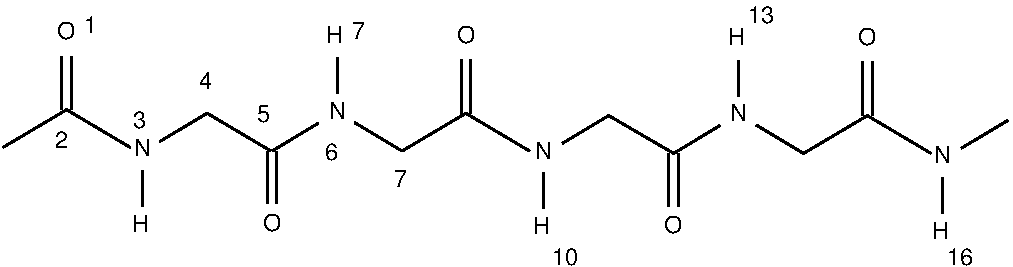
\includegraphics[width=100mm]{elicoidali.pdf}
\end{figure}}
\end{frame}

\subsection{Filamento $\beta$}
\begin{frame}
 \frametitle{Strutture secondarie}
  \framesubtitle{Filamento $\beta$}
\begin{itemize}
 \item Tipicamente si trovano in questa struttura secondaria sequenze di 5-10 AA.\pause
 \item Ammino acidi ingombranti e $\beta$ sostituiti si torvano spesso nel mezzo di un $\beta$ \emph{strand}.
\changeunitlength{0.05pt}
 \begin{figure}\begin{picture}(1300,1000)
\tetramethylenei{4==OH}{1==\bzdrv[c]{1==OH;4==(yl)};2SB==NH$_2$;2SA==H;3D==O}\end{picture}
 \begin{picture}(1500,800)\tetramethylenei{4==OH}{1W==\bzdrv[A]{2==(yl)};2SB==NH$_2$;2SA==H;3D==O}\end{picture}
 \begin{picture}(1500,800)\tetramethylenei{4==OH}{1W==\nonaheterov[bjge]{1==N}{1==H;3==(yl)};2SB==NH$_2$;2SA==H;3D==O}\end{picture}
 \begin{picture}(1100,800)\pentamethylene{5==OH}{2==OH;3SB==NH$_2$;3SA==H;4D==O}\end{picture}
 \begin{picture}(1100,800)\pentamethylene{5==OH}{2==\null;3SB==NH$_2$;3SA==H;4D==O}\end{picture}
 \begin{picture}(1100,900)\hexamethylenei{6==OH}{3A==\null;4SB==NH$_2$;4SA==H;5D==O}\end{picture}\end{figure}
\end{itemize}
\end{frame}
\begin{frame}\begin{figure}
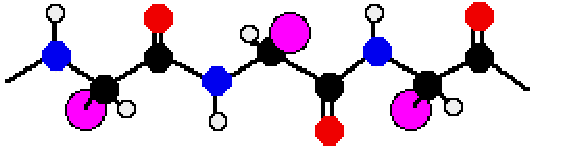
\includegraphics[scale=0.4]{bstrand.pdf}
\end{figure}
\begin{itemize}
\pause \item L'amminoacido prolina si trova solitamente alle estremità del $\beta$ filamento.
\pause \item Nonostante la nomenclatura di Nastro $2_7$, i filamenti $\beta$ non formano legami ad idrogeno tra un amminoacido ed il successivo. 
\pause \item Perciò non si osservano isolati ma solo all'interno di strutture supersecondarie: i foglietti $\beta$.
\pause \item Si indicano con una freccia dal N teminale al C terminale.
\end{itemize}

\end{frame}

\subsection{Elica $3_{10}$}
\begin{frame}
 \frametitle{Strutture secondarie}
  \framesubtitle{Elica $3_{10}$}
\begin{columns}
      
      \column{0.6\linewidth}
\begin{itemize}
\item L'elica $3_{10}$ si osserva raramente.
\pause\item Si osserva alle estremità delle $\alpha$ eliche.
\pause\item È un'elica destrorsa.
\pause\item I carbonili ed i legami ad idrogeno non sono ben allineati con l'asse. 
\item Le interazioni di van der Waals lungo l'asse causano repulsione.
\item Le catene laterali sono sovrapposte producendo repulsione sterica.
\end{itemize} \column{0.4\linewidth}
\begin{figure}
\begin{picture}(400,600)
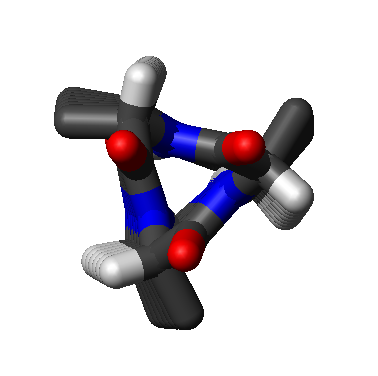
\includegraphics[scale=0.25]{310_helix_topview.png}
\end{picture}\caption{Vista dall'alto di una elica $3_{10}$ di poli-alanina. \tiny{immagine da Wikimedia.}}

\end{figure}\end{columns}
\end{frame}

\subsection{Elica $3.6_{13}$ - $\alpha$ elica}
\begin{frame}
 \frametitle{Strutture secondarie}
  \framesubtitle{Elica $3.6_{13}$ - $\alpha$ elica}

\begin{itemize}
\item L'$\alpha$ elica è la struttura secondaria più frequente nelle proteine globulari, trovata nel $32\%-38\%$ degli amminoacidi.
\pause \item È lunga mediamente 10 AA.
\pause \item È un'elica destrorsa.
\pause \item I dipoli dei legami peptidici sono quasi perfettamente allineati. 
\pause \item Gli idrogeni ammidici sono rivolti verso l'N terminale.
\end{itemize}\end{frame}\begin{frame}\begin{columns}
      \column{0.6\linewidth}
\begin{itemize}
\item Il raggio interno dell'elica permette interazioni di van der Waals favorevoli. 
\item Le catene laterali sono ben sfalsate per minimizzare le repulsioni steriche.

\end{itemize} \column{0.4\linewidth}\pause \vskip -10pt 
\begin{figure}
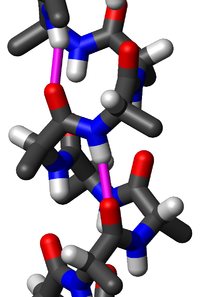
\includegraphics[scale=0.5]{alpha_helix.png}\caption{Vista laterale di una $\alpha$ elica di poli-alanina. \tiny{immagine da Wikimedia.}}
\end{figure}
\end{columns}
\end{frame}

\subsection{Elica $4.1_{16}$ - $\pi$ elica}
\begin{frame}
 \frametitle{Strutture secondarie}
  \framesubtitle{Elica $4.1_{16}$ - $\pi$ elica}
\begin{itemize}
\item La $\pi$ elica è estremanmente rara nelle proteine.
\item Come la elica $3_{10}$ si osserva alle estremità delle $\alpha$ eliche.
\pause \item Gli angoli $\psi$ e $\phi$ si trovano al limite di un minimo di energia potenziale della mappa di Ramachandran.
\item L'angolo $\tau$ cioè l'angolo $N-C\alpha-C'$ è forzato ad essere più aperto: 114.9° invece di 109.5°.
\item È un'elica destrorsa, solo la poli-glicina può dare $\pi$ elica sinistrorsa.
\end{itemize}\end{frame}\begin{frame}\begin{columns}
      \column{0.6\linewidth}
\begin{itemize}
\item Il raggio interno dell'elica \emph{non} permette interazioni di van der Waals favorevoli. 
\item Le catene laterali sono più sfalsate che in una elica $3_{10}$ ma meno di una $\alpha$ elica.
\end{itemize}\column{0.4\linewidth}\vskip -10pt \pause 
\begin{figure}
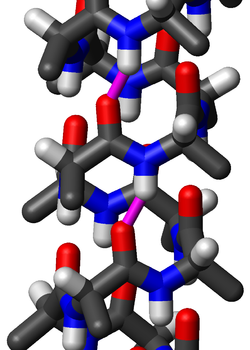
\includegraphics[scale=0.4]{pi_helix.png}\caption{Vista laterale di una $\pi$ elica di poli-alanina. \tiny{immagine da Wikimedia.}}
\end{figure}\end{columns}
\end{frame}

\section{Strutture supersecondarie}
\subsection{Motivi \& Domini}
\begin{frame}
 \frametitle{Strutture supersecondarie}
  \framesubtitle{Motivi \& Domini}
\begin{description}
\item [{Motivo strutturale}] organizzazione spaziale costituita da diversi elementi di struttura secondaria e dalle connessioni che li uniscono
\pause \item [{Motivo-Sequenza o Motivo funzionale}] sequenza di AA con una specifica funzione biochimica
\end{description}
\pause In questa presentazione si intende col termine \emph{motivo} il primo significato.
\begin{itemize}
 \item I vari elementi costituenti il motivo-sequenza possono essere discontinui ossia ci si può riferire a 
più sequenze sparse in una proteina e costituenti un preciso motivo-sequenza.
\end{itemize}
\end{frame}
\begin{frame}
Spesso alla parola motivo si attribuisce erroneamente il significato di dominio:
\begin{description}
\item [Dominio] una parte di proteina che può ripiegarsi in modo stabile anche se isolata in soluzione.
\end{description}\pause 
\begin{itemize}
\item Alcuni motivi, che verranno illustrati in seguito, costituiscono spesso un dominio. Ad esempio: 
\begin{itemize}
 \item il fascio a 4 eliche o \emph{four helix bundle}
 \item il  ripiegamento Rossmann
 \item la chiave greca
\end{itemize}\pause 
 \item Alcuni domini costituiti di pochi AA possono non contenere elementi di struttura secondaria.
\end{itemize}

\end{frame}

\begin{frame}
\begin{itemize}
 \item \textsc{Domini Alfa} - costituiti di $\alpha$ eliche.
\pause  \item \textsc{Domini Beta} - costituiti di $\beta$ filamenti.
\pause  \item \textsc{Domini Alfa/Beta} - costituiti da $\beta$ filamenti connessi da eliche.
\pause  \item \textsc{Domini Alfa+Beta} - costituiti da regioni $\alpha$ e $\beta$ separate.
\pause  \item \textsc{Domini reticolati} - costituiti da una povera struttura secondaria ma stabilizzati da ponti disolfuro o ioni metallici.
\end{itemize}

\end{frame}

\subsection{Motivi \itshape{all-$\alpha$} }
\begin{frame}
 \frametitle{Strutture supersecondarie}
  \framesubtitle{Fascio a 3 eliche - three helix bundle }
\begin{columns}
      
      \column{0.4\linewidth}
\begin{itemize}
 \item È il più piccolo dominio noto.
 \item Si osserva in proteine che legano l'actina e che legano il DNA.
\end{itemize}
      \column{0.65\linewidth}\vskip -10pt
\begin{figure}
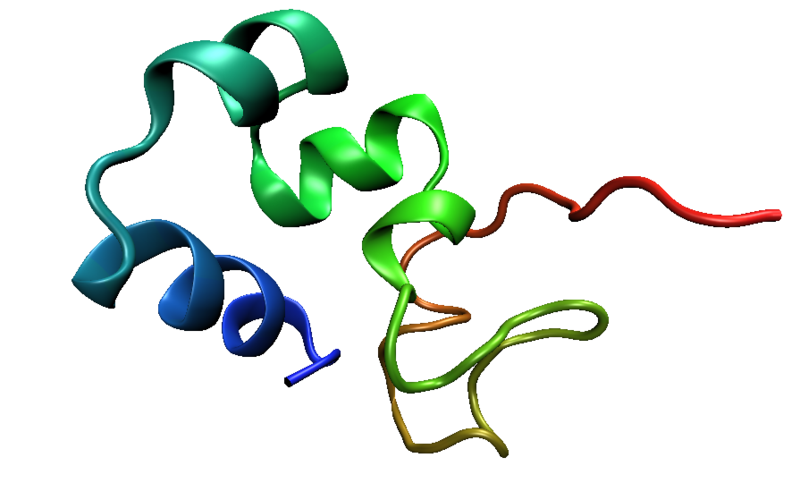
\includegraphics[scale=0.25]{3helix-bundle.png}\caption{Porzione terminale della Villina di gallina. Solo 36 AA. \tiny{immagine da Wikimedia.}}
\end{figure}
\end{columns}
\end{frame}


\begin{frame}
 \frametitle{Strutture supersecondarie}
  \framesubtitle{Fascio a 4 eliche - \itshape{four helix bundle}}

\begin{itemize}
 \item È un avvolgimento sinistrorso di eliche - \emph{coiled coil}.
 \item Lungo l'asse si ha una zona idrofobica stericamente proibita all'acqua.

 \item Solitamente le eliche affiancate sono antiparallele in modo da annullare i macrodipoli.\end{itemize}\end{frame}\begin{frame}
\begin{columns}
      
      \column{0.7\linewidth}
  
    \begin{itemize}
\uncover<2->{ \item Si osserva una periodicità eptadica: indicando con \emph{abcdefg} i gruppi di 7 AA \emph{a} e \emph{d} sono idrofobi, spesso 
isoleucina, leucina o valina, mentre i restanti sono idrofili.}
\uncover<3->{ \item Spesso paia di eliche affiancate sono stabilizzate da ponti salini che si stabiliscono per la presenza di AA ionici nelle posizioni \emph{e} e \emph{g}.
} \uncover<4->{ \item Queste strutture posso avere la funzione di trasporto dell'ossigeno, attacco ad acidi nucleici e trasporto elettronico. 
}\end{itemize}    
    
      \column{0.3\linewidth}\vskip -10pt
   \uncover<1->{   
       \begin{figure}
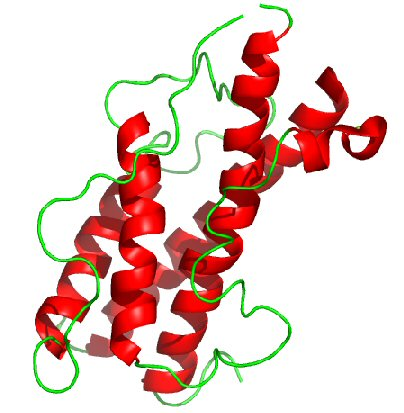
\includegraphics[scale=2]{4helix-bundle.jpg}\caption{Vista laterale di una four helix bundle. \tiny{immagine da chemistry.umeche.maine.edu}}
\end{figure} }
      
    \end{columns}

\end{frame}

\begin{frame}
\frametitle{Strutture supersecondarie}
  \framesubtitle{\itshape{Globin fold}}
\begin{columns}
      
      \column{0.6\linewidth}
\begin{itemize}
\uncover<2->{ \item Il \emph{Globin fold} è costituito da 8 $\alpha$ eliche indicate con le lettere A-H
 \item Gli assi delle eliche formano tra di loro angoli molto maggiori che nelle strutture \emph{coiled coil}.
 \item È il dominio che lega il gruppo \textsc{eme}.}
\end{itemize} 
     \column{0.45\linewidth}\vskip -10pt
\uncover<1->{
\begin{figure}
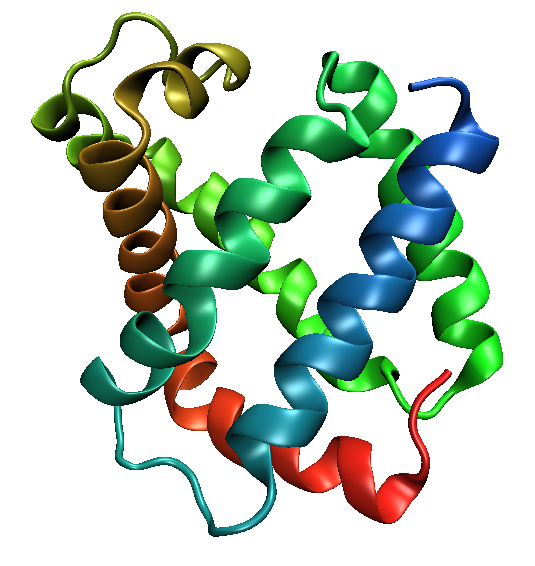
\includegraphics[scale=0.25]{globin-fold.png}\caption{Vista della Mioglobina. \tiny{immagine da Wikimedia.}}
\end{figure} } 
  \end{columns}

\end{frame}


\begin{frame}
 \frametitle{Strutture supersecondarie}
  \framesubtitle{Classificazione CATH}
La catalogazione CATH è una classificazione gerarchica dei motivi proteici.
\pause I primi livelli che vengono valutati da CATH:
\begin{enumerate}
 \item {\bf C}lass: il contenuto del motivo ($all-\alpha$\ldots)
\pause  \item {\bf A}rchitecture: un raggruppamento di topologie con caratterisctiche strutturali in comune 
\pause  \item {\bf T}opology: alta somiglianza strutturale ma senza omologia
\pause  \item {\bf H}omologous superfamily: strutture simili dovute ad ascendenza comune
\end{enumerate}
\pause \htmladdnormallink{http://www.cathdb.info}{http://www.cathdb.info}
\end{frame}

\begin{frame}
 \frametitle{Strutture supersecondarie}
  \framesubtitle{Classificazione CATH $all-\alpha$}
\begin{columns}
      \column{0.45\linewidth}
 \begin{figure}\begin{picture}(650,650)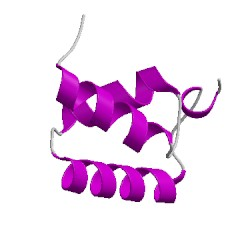
\includegraphics[scale=0.3]{cath-a1.jpeg}\end{picture}\caption{ Orthogonal Bundle}\end{figure}
\pause \begin{figure}\begin{picture}(260,260)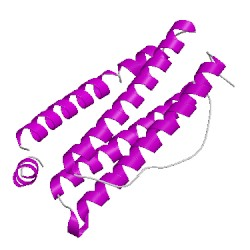
\includegraphics[scale=0.2]{cath-a2.jpeg}\end{picture}\caption{Up-down Bundle }\end{figure}\column{0.45\linewidth}
\pause \begin{figure}\begin{picture}(650,650)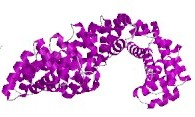
\includegraphics[scale=0.5]{cath-a3.jpeg}\end{picture}\caption{Alpha Horseshoe }\end{figure}
\pause \begin{figure}\begin{picture}(260,260)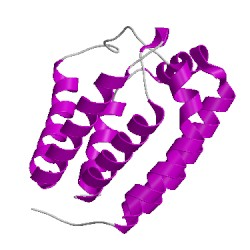
\includegraphics[scale=0.2]{cath-a4.jpeg}\end{picture}\caption{Alpha solenoid }\end{figure}\column{0.25\linewidth}
\pause \begin{figure}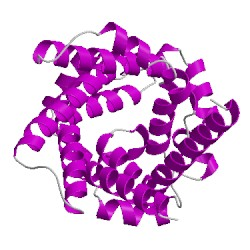
\includegraphics[scale=0.25]{cath-a5.jpeg}\caption{Alpha/alpha barrel}\end{figure}
\end{columns}
\end{frame}


\subsection{Motivi \itshape{all-$\beta$}}
\begin{frame} \frametitle{Strutture supersecondarie}
  \framesubtitle{Motivi \itshape{all-$\beta$}}
\begin{itemize}
 \item La maggior parte dei filamenti $\beta$ sono accoppiati ad altri filamenti stabilizzandosi così con la formazione di legami ad idrogeno.
 \pause  \item $\beta$ \emph{strands} adiacenti si allineano in modo tale che i rispettivi C$\alpha$ siano adiacenti e che le rispettive catene laterali puntino nella stessa direzione.
\pause \item Le catene laterali puntano circa perpendicolarmente al piano dei legami ad idrogeno ed alternatamente nei due versi.
\pause  \item A causa della chiralità degli AA, non si ha la conformazione estesa al massimo ma si ha una torsione.\end{itemize}\end{frame}\begin{frame}
\begin{itemize} \item Si possono avere difetti nella struttura dei legami ad idrogeno come un rigonfiamento $\beta$ o $\beta$ \emph{bulge}.
\begin{columns}
      
      \column{0.5\linewidth}\begin{figure}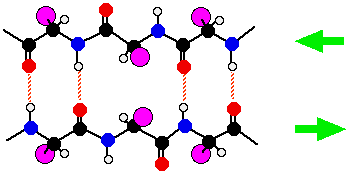
\includegraphics[scale=0.3]{bhairpin.png}\caption{Due filamenti $\beta$ antiparalleli.}\end{figure}
\column{0.5\linewidth}\begin{figure}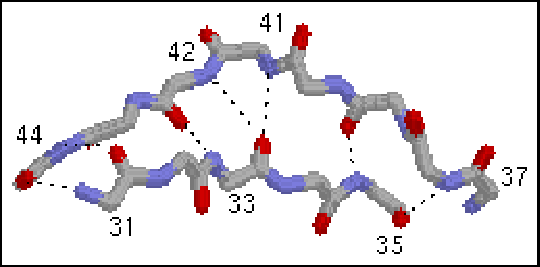
\includegraphics[scale=0.5]{bbulge.pdf}\caption{Un $\beta$ bulge.}\end{figure}
\end{columns}

\end{itemize}\end{frame}\begin{frame}

\begin{columns}
      
      \column{0.7\linewidth}
\begin{itemize}
 \item I filamenti accoppiati possono essere paralleli o antiparalleli.
 \item Il foglietto $\beta$ antiparallelo
\begin{itemize}
\pause   \item forma i legami ad H su un piano.
 \pause  \item ogni AA fa 2 legami ad idrogeno entrambi con il rispettivo AA sull'altro filamento formando il cosiddetto \emph{accoppiamento vicino}.
\end{itemize}
\end{itemize}\column{0.35\linewidth}
\begin{figure}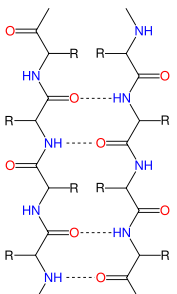
\includegraphics[scale=0.5]{beta_sheet_antiparallel.png}\caption{Due filamenti $\beta$ anti paralleli.}\end{figure}\end{columns}
\end{frame}\begin{frame}
\begin{columns}
      \column{0.9\linewidth}
\begin{itemize}
  \item Il foglietto $\beta$ parallelo \begin{itemize}
\pause  \item è meno stabile a causa dei suoi legami ad H.
\pause   \item ogni AA fa 2 legami ad H: uno con l'AA precedente al rispettivo AA sull'altro filamento ed uno col successivo formando il cosiddetto \emph{accoppiamento largo}.
\pause   \item i filamenti sono distanti nella sequenza amminoacidica, il collegamento più comune è una $\alpha$ elica.
\end{itemize} \end{itemize}
\begin{figure}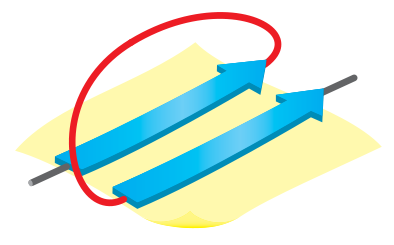
\includegraphics[scale=0.35]{betasheet-parallel.png}\caption{Un collegamento destrorso.}\end{figure}

\column{0.2\linewidth}\begin{figure}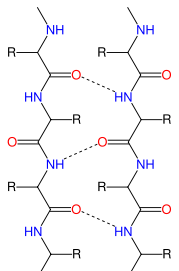
\includegraphics[scale=0.35]{beta_sheet_parallel.png}\caption{Due filamenti $\beta$ paralleli.}\end{figure}  \end{columns}
\end{frame}

\begin{frame}
La nomenclatura\citep{richardsonbeta} per la topologia dei $\beta$ foglietti è illustrata in questa figura.
\begin{figure}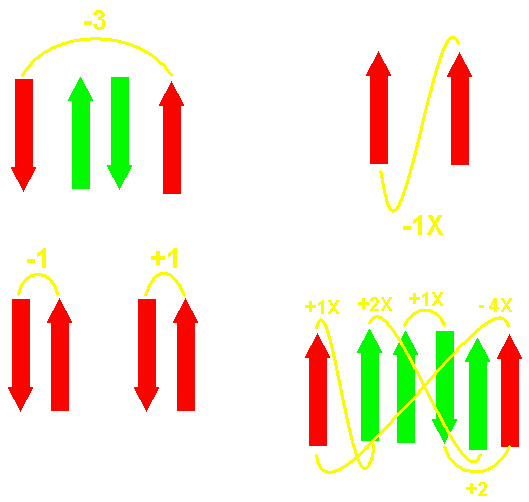
\includegraphics[scale=0.25]{betasheetcodici.png}\end{figure}  
\end{frame}

\begin{frame}
 \frametitle{Strutture supersecondarie}
  \framesubtitle{$\beta$ harpin}
\begin{columns}
      
      \column{0.8\linewidth}
\begin{itemize}
 \item La $\beta$ \emph{hairpin} si può indicare anche con unità $\beta - \beta$.
\pause  \item È costituita da 2 $\beta$ filamenti appaiati antiparalleli e collegati da un \emph{loop} di 3-5 AA.
\pause  \item Con il termine $\beta$ \emph{hairpin} si può intendere anche un tipo di \emph{loop}.
\end{itemize}
  \setbeamercolor{uppercolor}{fg=white, bg=black}
  \setbeamercolor{lowercolor}{fg=white, bg=blue!50!black}
\pause   \begin{beamerboxesrounded}[upper=uppercolor, lower=lowercolor, shadow=true]
    {I \emph{loop}}
    I \emph{loop} sono elementi di struttura secondaria che invertono il verso della catena. Se si forma un legame ad H tra l'amminoacido $n$ e l'$n+3$ si chiama $\beta$ \emph{turn}. Se si forma tra $n$ e $n+2$ si chiama $\gamma$ \emph{turn}. 
  \end{beamerboxesrounded}
\column{0.3\linewidth}\vskip -10pt
\begin{figure}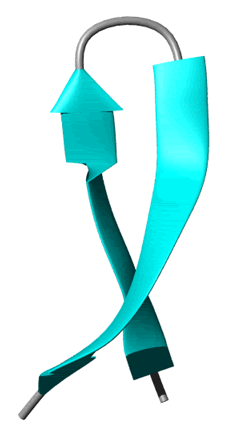
\includegraphics[scale=0.25]{beta_hairpin.png}\caption{Una $\beta$ \emph{hairpin}. \tiny{immagine da Wikimedia.}}\end{figure}  
  \end{columns}
\end{frame}

\begin{frame}
\frametitle{Strutture supersecondarie}
  \framesubtitle{Chiave greca - \itshape{Greek key} - \itshape{Meander}}
\begin{itemize}
 \item La chiave greca consiste in 4 filamenti $\beta$.
 \item Tre dei quattro filamenti formano dei $\beta$ \emph{hairpin} mentre l'ultimo è affiancato al primo e collegato con un lungo \emph{loop}.
\pause  \item La nomenclatura secondo Richardson è -3+1+1 o -1-1+3.
\end{itemize}   \begin{figure}
\centering
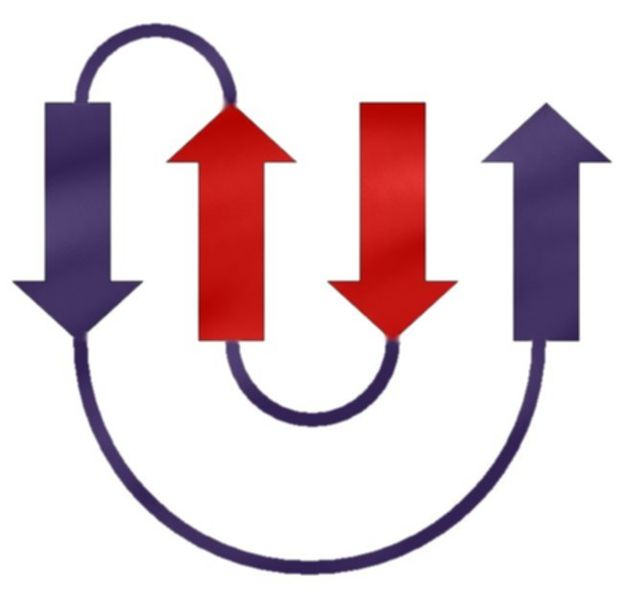
\includegraphics[scale=0.7]{greek_key.jpg}\end{figure}
\end{frame}


\begin{frame}\frametitle{Strutture supersecondarie}
  \framesubtitle{\itshape{Jellyroll}}
Un \emph{Jellyroll} è una chiave greca con un avvolgimento aggiuntivo.   \begin{figure}
\centering
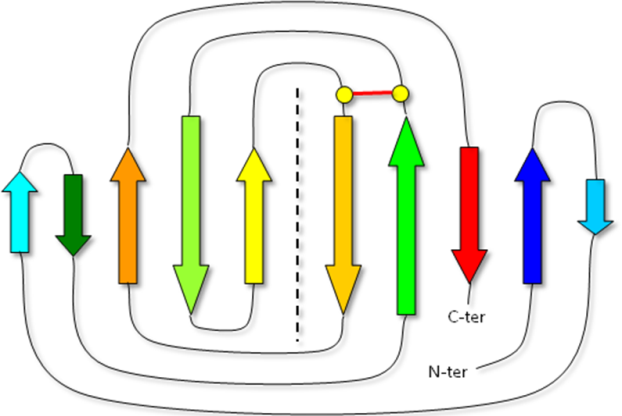
\includegraphics[scale=0.25]{jellyroll.png}
\end{figure}

\end{frame}



\begin{frame}
\frametitle{Strutture supersecondarie}
  \framesubtitle{\itshape{$\beta$ helix}}\begin{columns}
      \column{0.5\linewidth}
Una $\beta$ elica è formata da filamenti $\beta$ paralleli avvolti in una struttura elicoidale a 2 (in cui per effetto idrofobico si affacciano 2 foglietti $\beta$ paralleli ricchi di glicina) o 3 facce.\\ È stata osservata sia destrorsa sia sinistrorsa.
  \column{0.55\linewidth} \vskip -10pt \begin{figure}
\centering
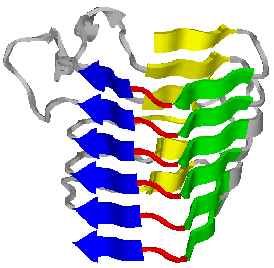
\includegraphics[scale=0.45]{betaHelix.png}\caption{Una $\beta$ elica facente parte del Pectate Lyase C dalla Erwinia chrysanthemi (PDB ID 1pcl) \tiny{immagine da groups.csail.mit.edu}}
\end{figure} \end{columns}
\end{frame}
\begin{frame}
\frametitle{Strutture supersecondarie}
  \framesubtitle{\itshape{$\beta$ \emph{trefoil}}}
\begin{columns}
      \column{0.5\linewidth}
Un $\beta$ \emph{trefoil} è costituito da 12 filamenti $\beta$ raggruppati in 3 subunità beta-beta-beta-loop-beta (trifoglio).\\
La struttura finale ha un asse di simmetria ternario.\column{0.55\linewidth}
\begin{figure}
\centering
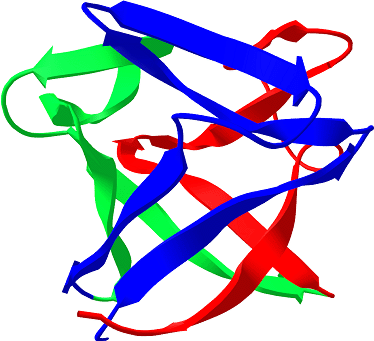
\includegraphics[scale=0.35]{trefoil.png}\caption{Un $\beta$ \emph{trefoil} facente parte del Human Basic Fibroblast Growth Factor (PDB ID 1bff) \tiny{immagine da groups.csail.mit.edu}}
\end{figure} \end{columns}
\end{frame}
\begin{frame}
\frametitle{Strutture supersecondarie}
  \framesubtitle{\itshape{$\beta$ \emph{propeller}}}\begin{columns}
      \column{0.35\linewidth}
Un $\beta$ propeller è costituito da 4 a 8 unità di foglietti $\beta$ antiparalleli disposti attorno ad un asse principale.
Tipicamente ciascuna unità è formata da 4 filamenti torti in modo da avere il primo perpendicolare al quarto.
 \column{0.75\linewidth}  \vskip -10pt \begin{figure}
\centering\begin{picture}(1000,1350)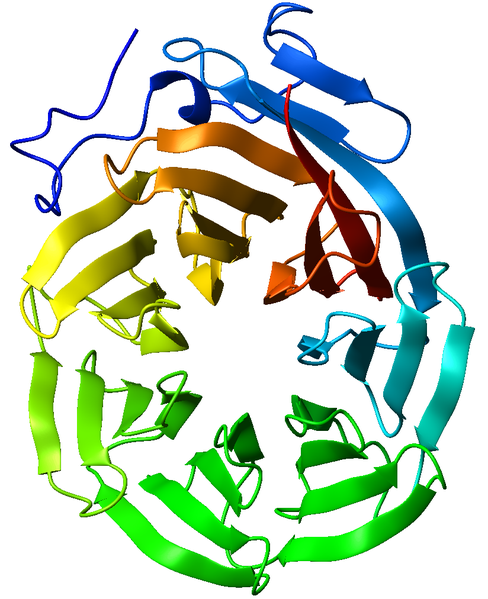
\includegraphics[scale=0.25]{betapropeller.png}
          \end{picture}\\ Un $\beta$ \emph{propeller} parte del Tup1 (co-repressore trascrizionale nel lievito) \tiny{immagine da Wikimedia}
\end{figure} \end{columns}
\end{frame}
\begin{frame}
\frametitle{Strutture supersecondarie}
  \framesubtitle{\itshape{$\beta$ \emph{sandwich}}}
\begin{itemize}
\item Spesso i $\beta$ foglietti antiparalleli hanno una faccia con residui idrofobi ed una con residui idrofili.
\pause  \item Per impaccare le facce idrofobe all'interno del \emph{core} proteico si può formare un $\beta$ \emph{sandwich}.
\pause  \item Nel $\beta$ \emph{sandwich} due foglietti $\beta$ formati da più filamenti $\beta$ si affacciano come in un \emph{sandwich}.
\item Spesso l'angolo tra la direzione dei filamenti nei due foglietti è un angolo retto.
\end{itemize}
\end{frame}
\begin{frame}
\frametitle{Strutture supersecondarie}
  \framesubtitle{\itshape{$\beta$ barile}}
\begin{columns}
      \column{0.7\linewidth}
\begin{itemize}
 \item L'altro modo in cui dei foglietti $\beta$ si possono associare per dare un \emph{core} idrofobico è formando un $\beta$ barile.
\pause   \item La differenza col $\beta$ \emph{sandwich} è che nel barile i filamenti alle estremità sono collegati da legami ad idrogeno formando un cilindro.
\pause   \item Per formare questo motivo sono necessari almeno 6 filamenti.
\end{itemize}\column{0.4\linewidth}
 \begin{figure}
\centering
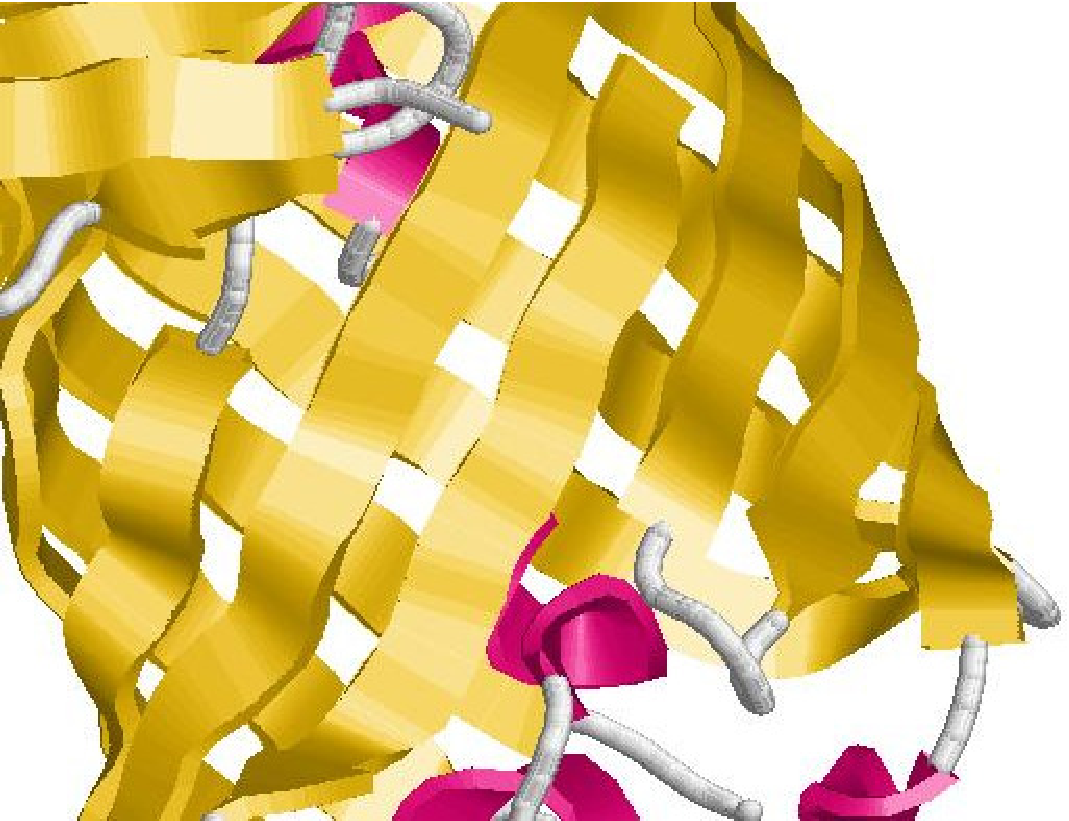
\includegraphics[scale=0.22]{betabarrel.pdf}\caption{Un $\beta$ barile costituito da 11 filamenti $\beta$ facente parte della \emph{Green fluorescent protein}\citep{PDB}}\label{bbarrel}
\end{figure} 
\end{columns}
\end{frame}


\begin{frame}
 \frametitle{Strutture supersecondarie}
  \framesubtitle{Classificazione CATH $all-\beta$}
\begin{columns}
      \column{0.35\linewidth}
\begin{itemize}
 \item Ribbon
 \item Single Sheet
 \item Roll
 \item Beta Barrel
 \item Clam
 \item Sandwich
 \item Distorted Sandwich
\end{itemize}

\column{0.35\linewidth}\begin{itemize}
 \item Trefoil
 \item Orthogonal Prism
 \item Aligned Prism
 \item 3-layer Sandwich
 \item 3 Propellor
 \item 4 Propellor
 \item 5 Propellor
\end{itemize}
\column{0.35\linewidth}
\begin{itemize}
 \item 6 Propellor
 \item 7 Propellor
 \item 8 Propellor
 \item 2 Solenoid
 \item 3 Solenoid
 \item Beta Complex
\end{itemize}
\end{columns}
\end{frame}

\subsection{Motivi $\alpha/\beta$}
\begin{frame}
\frametitle{Strutture supersecondarie}
  \framesubtitle{$\beta-\alpha-\beta$}
\begin{itemize}
\item Il ripetersi di strutture $\beta-\alpha-\beta$ è molto comune.
\pause   \item Può essere destrorso (comune) o sinistrorso (molto raro).
\pause   \item I filamenti sono paralleli.
\pause  \item La ripetizione $\beta-\alpha-\beta-\alpha-\beta$ è comune nelle proteine che legano i nucleotidi e viene chiamato \emph{Rossman Fold}.
\pause  \item La stabilità di questa struttura si può intuire osservando la complementarietà delle catene laterali dei foglietti e di quelle delle eliche
\end{itemize}
\end{frame}

\begin{frame}
\frametitle{Strutture supersecondarie}
  \framesubtitle{$\alpha/\beta$ horseshoe}
\begin{figure}
\centering
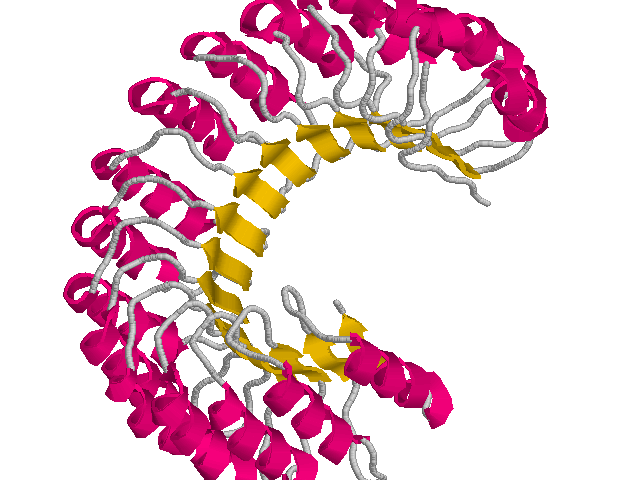
\includegraphics[scale=0.3]{horseshoe.png}\caption{Un $\alpha/\beta$ \emph{horseshoe} - zoccolo di cavallo (PDB ID 1bnh)\citep{PDB}}\label{bbarrel}
\end{figure} 
\end{frame}

\begin{frame}
\frametitle{Strutture supersecondarie}
  \framesubtitle{Rossmann fold}
\begin{columns}
      \column{0.35\linewidth}
\begin{itemize}
 \item 6 coppie $\alpha\beta$ non possono formare un barile ma solamente un foglietto parallelo con su entrambi i lati 3 $\alpha$ eliche.
 \item Il Rossmann fold si osserva nei leganti dei nucleotidi.
\end{itemize}
\column{0.7\linewidth}
\begin{figure}
\centering\begin{picture}(1000,1350)
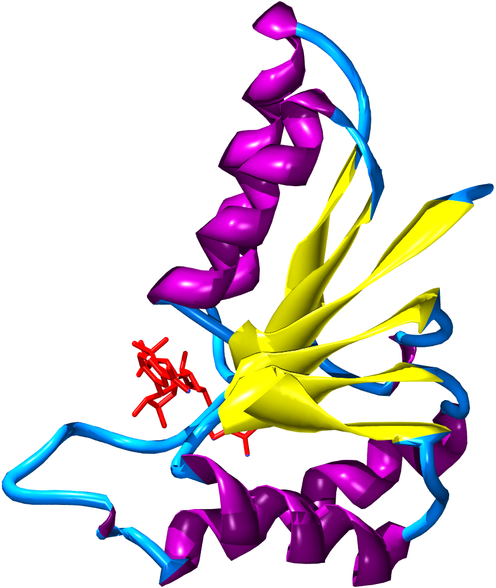
\includegraphics[scale=0.25]{Rossman_fold.png}          \end{picture}\caption{Un Rossmann fold costituito da 6 filamenti $\beta$ e 4 eliche $\alpha$(PDB ID 2FM3)}


\end{figure} \end{columns}
\end{frame}
\begin{frame}
\frametitle{Strutture supersecondarie}
  \framesubtitle{$\alpha/\beta$ barile}\begin{columns}
      \column{0.65\linewidth}
\begin{itemize}
\item Un $\alpha/\beta$ barile è costituito da filamenti $\beta$ paralleli collegati da eliche $\alpha$.
\pause  \item Il caso più famoso è il \emph{TIM-barrel} costituito da 8 unità $\alpha\beta$ anche indicato con $(\alpha\beta)_8$.
\pause  \item Nell'immagine a lato l'$\alpha/\beta$ barile appare cavo ma in realtà è occupato dalle catene laterali in gran parte idrofobe del $\beta$ foglietto.

\end{itemize} \column{0.45\linewidth}\begin{figure}
\centering
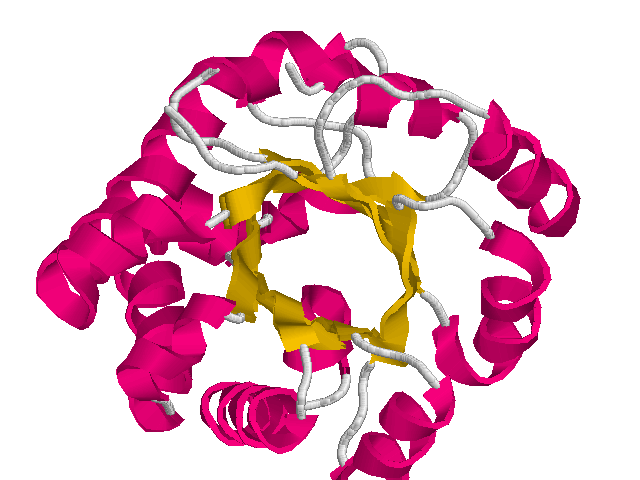
\includegraphics[scale=0.22]{ab-barrel.png}\caption{Un $\alpha/\beta$ \emph{barrel}. Una delle due unità della triosofosfato isomerasi (PDB ID 2x1s)\citep{PDB}}\label{bbarrel}
\end{figure} \end{columns}
\end{frame}




\subsection{Motivi $\alpha+\beta$}
\begin{frame}
\frametitle{Strutture supersecondarie}
  \framesubtitle{Motivi $\alpha+\beta$}
\begin{itemize}\item Ci sono 2 tipi principali di motivi $\alpha+\beta$\citep{aplusb}:
\begin{itemize}
\pause   \item $\alpha-\beta$ \emph{sandwich} in cui le strutture $\alpha$ e $\beta$ costituiscono strati differenti e si osserva il ripetrsi del motivo $\beta-\alpha-\beta$. È il ripiegamento più stabile dei due.
\pause   \item $\alpha-\beta$ \emph{rolls} contiene meno eliche e i foglietti $\beta$ si arrotolano per formare una culla per la $\alpha$ elica.
\end{itemize}

\end{itemize}
\end{frame}

\begin{frame}
 \frametitle{Strutture supersecondarie}
  \framesubtitle{Classificazione CATH $\alpha$ $\beta$ }
\begin{columns}
      \column{0.35\linewidth}
\begin{itemize}
 \item Roll
 \item Super Roll
 \item Alpha-Beta Barrel
 \item 2-Layer Sandwich
 \item 3-Layer(aba) Sandwich
\end{itemize}
\column{0.35\linewidth}
\begin{itemize}
 \item 3-Layer (aab) Sandwich
 \item 3-Layer(bba) Sandwich
 \item 3-Layer(bab) Sandwich
 \item 4-Layer Sandwich
 \item Alpha-beta prism
\end{itemize}\column{0.35\linewidth}\begin{itemize}
 \item Box
 \item 5-stranded Propeller
 \item Alpha-Beta Horseshoe
 \item Alpha-Beta Complex
 \item Ribosomal Protein L15; Chain: K; domain 2
\end{itemize}
\end{columns}
\end{frame}


\subsection{Motivi reticolati}
\begin{frame}
\frametitle{Strutture supersecondarie}
  \framesubtitle{Domini reticolati}
\begin{itemize}\item Piccole proteine ricche in legami disolfuro danno luogo a domini reticolati.
\pause   \item Sono stabilizzati principalmente dai legami disolfuro e secondariamente da legami ad idrogeno ed interazioni idrofobiche. 
\pause   \item Possono essere classificate in 41 gruppi in base alla struttura. \citep{disulfide}
\end{itemize}
\end{frame}


\bibliography{bibliography.bib}
\bibliographystyle{plainnat}
\end{document}
